%===============================================================================
\chapter{Control logic design}\label{ch03}
%===============================================================================
%
\begin{quote}
    \begin{flushright}
        \textit{Any sufficiently advanced technology \\
        is indistinguishable from magic.}\\
        \vspace{0.2cm}
        Arthur C. \citet{Clarke1968law3} \\
    \end{flushright}
\end{quote}
\vspace{1cm}

The design of the control logic and the formulation of the optimisation problem is described in this chapter. A brief introduction to model-base and model-free algorithms for flow control is provided, focusing on the two machine-learning-based algorithms used in this thesis: linear evolutionary algorithms and deep reinforcement learning.

\section{Turbulence flow control}

Turbulent flow control is a sub-field that intersects the study of turbulence and the application of control techniques. Three common strategies are found to control turbulence: aerodynamics shape optimisation, passive and active control. The reader is referred to Chapter~\ref{ch02} for an introduction to passive and active methods for heat transfer control in turbulent flows. Nonetheless, several other challenges are to be tackled, such as the proper selection of the flow control system (plant), meaningful sensing, the effective objective function or the control logic. In this following, a brief description of a general flow control problem is provided.

The mechanisms driving momentum and energy transports targeted by flow-control strategies greatly depend on the laminar or turbulent regime on which the fluid flow develops. Besides the appreciable understanding of turbulence, it is still hard to agree on a single, self-sustained definition of turbulence. The classic and complete definition by \citet{Bradshaw1971turbulence} reads,
%
\begin{quote}
    “turbulence is a three-dimensional time-dependent motion in which vortex stretching causes velocity fluctuations to spread to all wavelengths between a minimum determined by viscous forces and a maximum determined by the boundary conditions of the flow. It is the usual state of fluid motion except at low Reynolds numbers”.
\end{quote}
%
This rationale provides three main pillars upon which any turbulence flow control must build: the chaotic nature of turbulence, the existence of a wide range of scales in both space and time, and the three-dimensionality of the phenomena. Since the long-established study by \citet{Richardson1920}, and its extension by \citet{Kolmogorov1941}, it is well-known that the large-scale motion produces the energy that progressively flows through the spectral pipeline to the smallest eddies where it is dissipated into heat. In the particular case of a turbulent boundary layer, an effective control strategy to reduce turbulent fluxes tends to interrupt a self-sustained cycle involving near-wall turbulent structures \citep{hamilton1995,Jimenez1999, schoppa2002}, such as the opposition control for streak suppression \citep{Choi1994}. Hence, the cancellation or exacerbation of large-scale turbulent structures could effectively control physical phenomena such as reduction of skin-friction drag or heat and mixing enhancement.

The design of an optimal control strategy for turbulent flows is an ambitious venture. As discussed by \citet{cornejomacedaPhD}, there are three factors that affect the design of the turbulence flow control problem and its optimality:
%
\begin{itemize}
    \item \textbf{High-dimensionality}: the existence of a wide range of scales in time and space sets a strong requirement for flow reconstruction from simulation or experimental data. High time and space resolution data is required, rendering the problem sensing very costly;
    \item \textbf{Time-delayed response}: mainly related to the a non-negligible transient time between sensing and actuation command;
    \item \textbf{Frequency crosstalk}: modelling and predicting the flow becomes critical when there is a nonlinear interaction between modes.
\end{itemize}
%
Regarding the control logic, literature distinguishes between model-based and model-free algorithms. On the one hand, the model-based approach has shown its effectiveness when the flow control configurations can be modelled based on first- or second-order dynamics \citep{Rowley2006control}. Based on linear control theory, the main idea behind model-based algorithms is linearising the flow dynamics around a specific state of interest \citep{Kim2007linearcontrol,Sipp2010linearcontrol}. It is also common to project the dynamics on a reduced-order subspace composed of several dominant non-normal global stability eigenmodes \citep{akervik2007galerkin}. Some successful examples of model-based control are the opposition control \citep{Choi1994, Fukagata2003oppcontrol}, two-frequency crosstalk \citep{Glezer2005control,luchtenburg2009galerkin}, phasor control to stabilise oscillations \citep{pastoor2008control}, and quasi-steady response to quasi-steady actuation \citep{Pfeiffer2018robustcontrol}, to name a few. Notwithstanding, model-based approaches still grapple with turbulent flows, since linear control theory omits nonlinear interactions among modes \citep{BruntonNoack2015review}. Furthermore, the experimental investigation of turbulence control comes along with several technological constraints, such as the placement, quantity and type of sensors and actuators, which are regularly outlined from experience and engineering wisdom \citep{Cattafesta2011revFC}. The hitherto available measurement techniques provide a sparse representation of the flow state either due to insufficient time or spatial resolution. These additional constraints make model-based approaches often unpractical for in-time control \citep{cornejomacedaPhD}.

Model-free approaches, on the other hand, can derive optimised actuation commands for a certain flow configuration with a sparse representation of the state. These algorithms do not rely on any simplified or reduced-order model but consider the flow system as a black-box model that only attends to the actuation command and the sensor signals. Deriving optimal control laws based on model-free approaches is a complex enterprise, which requires the utilization of sophisticated regression techniques, based for instance on machine learning algorithms. Still, the non-convexity of the feasible solution space for the actuation design also challenges the model-free optimisation of turbulence control. In experiments, the problem is often simplified by selecting a reduced number of actuation parameters with adaptive variations either based on temporal evolution or sensor signal. Common model-free strategies for turbulence control are the evolutionary algorithms \citep{Koumoutsakos2001evolcontrol} and genetic algorithms \citep{Benard2016ga}, the extremum and slope-seeking control method \citep{Krstic2000extremumseek, Becker2007extseek, Gelbert2012extseek} and physics-based methods \citep{pastoor2008control,Zhang2004control}. 

The control logic proposed in the different analyses of this thesis is based on model-free approaches. The application of machine learning techniques to the field of fluid mechanics and flow control is a trending topic nowadays that continuously updates the state of the art. The comparative assessment presented in the Paper 4 of this thesis deals with two of the most prominent model-free control techniques from the machine learning literature, namely Reinforcement Learning (RL) \citep{sutton2018reinforcement} and Genetic Programming (GP) \citep{Koza1994gp}. On the other hand, the experimental flow control study described in Paper 5 employs linear generic algorithm control (LGAC) \citep{Benard2016ga} to find optimal open-loop control laws for heat transfer enhancement in a turbulent boundary layer. A brief description of the fundamentals of evolutionary algorithms and reinforcement learning is provided at the end of this chapter.

%------------------------------------------------------------------------------------------------
\subsection{Flow control as an optimisation problem}\label{ss:optproblem}
Solving the flow control problem based on a model-free algorithm is not a simple task. A common approach is to formulate it as an optimisation problem, in which the control law for each actuator is optimised based on a certain objective function while complying with either physical or technological constraints. The fluid system to be controlled, referred to as \textit{plant} from now on, is treated as a black-box model. The plant can represent several scenarios such as \citep{cornejomacedaPhD},
%
\begin{itemize}
    \item \textbf{Dynamical system}: defined as a system of equations, such as for instance the differential equations describing the Lorenz system.
    \item \textbf{Numerical simulation}: the computational resolution of a discretised system of equations, such as the Euler equations, the Reynolds Average Navier Stokes, or the direct numerical simulation of the N-S equations. This kind of plant usually provides a complete image of the flow state with no noise or disturbances affecting the sensing or actuation command.
    \item \textbf{Real fluid flow in a controlled environment}: the flow configuration is replicated in a controlled facility such as wind tunnels, free jets in a laboratory environment, channels, etc. The realistic environment of the experiment comes alongside external noise and disturbance affecting the flow state itself, as well as the measurements.
    \item \textbf{Real fluid flow}: direct testing of industrial applications such as a car, an aircraft, a heat exchanger or a jet engine in real-life conditions;
\end{itemize}
%
The control of the plant is achieved by the utilisation of actuators, whose number and type will strongly depend on the flow configuration and the target of the optimisation. In Chapter~\ref{ch02}, several actuators used in heat transfer control applications are introduced, especially those under consideration in this thesis: plasma actuators and jets in crossflow. Besides their working principle, all the actuators aim at disturbing the flow in a certain way to exacerbate or cancel out the desired effect on the fluid flow. The actuation command is a vectorial quantity, $\bm{b}(t) = (b_1, \ldots ,b_{N_b})^T$, with as many elements as the number of actuators under consideration $N_b$. When the actuation command is driven by feedback information of the state, the control is said to be of the \textit{closed-loop} kind; otherwise, the actuation is commonly based on fixed or time-dependent parameter with no system information, which is known as \textit{open-loop} control. Both approaches are explored in this thesis, the former in Paper 4 and the latter in Paper 5. 

The following formulation of the flow control problem is presented in its most complete form, considering feedback information $\bm{s}$, actuation parameters $\bm{\theta}$ and time-dependent functions $\bm{h}$. The sensing information is a vectorial quantity, $\bm{s}(t) = (s_1, \ldots ,s_{N_s})^T$, with as many elements as sensors in use $N_s$. On the other hand, the number of control parameters $N_p$ and time-dependent functions $N_h$ is fully dependant on the problem at hand. We define a control parameter $\theta_i$ as a constant quantity affecting the controller somehow as could be the frequency or the duty cycle of a modulated flow, for example. Regarding the functions $\bm{h}(t)$, they are used to refer to time-dependent information that does not depend on the sensing, as it could be harmonic functions of a certain phenomenon. The actuation command is related to these three vectorial quantities as follows,
%
\begin{equation}
    \bm{b}(t) = \bm{K}(\bm{s}(t),\bm{h}(t);\bm{\theta})
\end{equation}
%
The function $\bm{K}: \mathbb{X} \mapsto \mathbb{K}$  maps the input space $\mathbb{X}$, comprising the parameters, sensors and harmonic functions, to the control-law space $\mathbb{K}$. 

The optimal $\bm{K}$ derives from the optimisation of a certain objective function. In fluid mechanics, the targeted objective functions in flow control problems usually relate to the minimization of drag, mixing enhancement, heat transfer enhancement or separation control, to name a few. The goal of the control problem is defined in the cost function $J$, which commonly decouples on physical phenomena on the plant $J_a$ and a penalisation term of the required energy for controlling such phenomena $J_b$,
%
\begin{equation}
    J = J_a(\bm{b}) + \alpha J_b(\bm{b})
\end{equation}

The cost function is a scalar quantity that depends on the performance of the control. From an optimisation standpoint, the flow control problem becomes a minimisation problem in which the optimal control $\bm{K^*}$ yields the minimum value of the cost function $J$ over the search space $\mathbb{K}$. The relevance of the penalisation term in the cost function can be customarily tuned by the parameter $\alpha$. A large value of $\alpha$ prioresses the energy consumption required by the actuation, which commonly leads to low, or even negligible, control intensity. The correct balance between both terms depends on the flow configuration under consideration and is commonly based on experience and engineering wisdom. Thus, the flow control problem reads as follows
%
\begin{equation}\label{eq:Optproblem}
    \begin{aligned}
        \bm{K}^{*} = \underset{{\bm{K} \in \mathbb{K}}}{\arg\min}~~ J(\bm{K})
    \end{aligned}
\end{equation}

This optimisation problem is a non-convex optimisation problem, which could be interpreted as a regression problem of the second kind since the optimal solution is not known. The distinction between regression models of the first and second kind was first introduced by \citet{Fisk1967reg}. The regression problems of the first kind are those in which a full representation of the plant is assumed by a transfer function $\bm{P}$ so that it is possible to relate the response of all the possible actions for every state. Hence, the regression problem consists of inverting the model of the plant, $\bm{P^{-1}}$, achieving a direct mapping of the sensors and the actuation command. Conversely, the regression problem of the second kind does not assume any knowledge of the plant dynamics. Since the optimal solution is unknown, this kind of problem relies just on the control performance, namely the cost function $J$. The interested reader is referred to the long-established work by \citet{Fisk1967reg} for a deep description of the regression of the second kind, and to the thesis by \citet{cornejomacedaPhD} for a more friendly and visual description of both problems.

% %%%%%%%%%%%%%%%%%%%%%%%%%%%%%%%%%%%%%%%%%%%%%%%%%%%%%%%%%%%%%%%%%%%%%%%%%%%%%%%%%%
\section{Reinforcement Learning}

\textit{Learning by doing} is, surely, the most intuitive, simple and common way of learning in nature and society. Like a kid practising how to ride a bike or a lion training for hunting, Reinforcement Learning (RL) is a computational approach to interactive learning. The RL learner, known as the agent, learns a mapping function between observations and actions with the specific target of maximising certain reward. This is a \textit{trial-and-error} process, through which the agent determines the intrinsic nature of the phenomena under control and, somehow, predicts the expected reward upon future actions. According to the categories proposed by \citet{BruntonNoackKoumoutsakos2020}, reinforcement learning is considered a \textit{semi-supervised learning} approach. Contrary to supervised learning, in which the labelled data is available to train the model, semi-supervised learning only counts on partially labelled data or, in the case of RL, on the interactions of the machine with the environment.  

This section introduces the essential principles of RL, its elements and the considered algorithm for training are introduced in this section. The herein explanation is mainly retrieved from the pioneering work by \citet{sutton2018reinforcement}, and the recent reviews on RL applied to fluid mechanics by \citet{Garnier2021RLrev} and \citet{Viquerat2021RLrev}. The curious reader is referred to these literature contributions for a profound understanding of this matter.

%---------------------------
\subsection{Basic elements, principles, and mathematical foundation}\label{ss:RLbasic}
%
Reinforcement learning is a class of mathematical methods for problem-solving based on decision-making \citep{sutton2018reinforcement}, which involve the goal-directed interactions of an agent with the environment \citep{BruntonNoackKoumoutsakos2020}. This interaction splits into (1) the observations from the environment, (2) the application of an action based on the previous observations, and (3) the quantification of the performance. Although RL models the interactions with the environment as a Markov decision process, similarly to dynamic programming \citep{Bellman1952dyprog}, there is no need to model the dynamics of the environment.

The typical learning loop for RL is illustrated in figure~\ref{fig:RL_loop} and executes as follows \citep{Viquerat2021RLrev}:
%
\begin{itemize}
    \item Assume the time instant $t$ at which the environment is defined by its state $s_t \in \mathcal{S}$;
    \item the agent commands an action $a_t \in \mathcal{A}$ based on the observation of the current state, which could be a full $s_t$ or partial observation $w_t$ (subset of $s_t$, taken from sensing for instance);
    \item the environment evolves from $s_t$ to $s_{t+1} \in \mathcal{S}$ upon the action of the agent;
    \item the agent receives a reward $r_t \in \mathcal{R}$ for the previous actuation, and a new observation $s_{t+1}$ (or $w_{t+1}$).
\end{itemize}
%
\begin{figure}
    \centering
    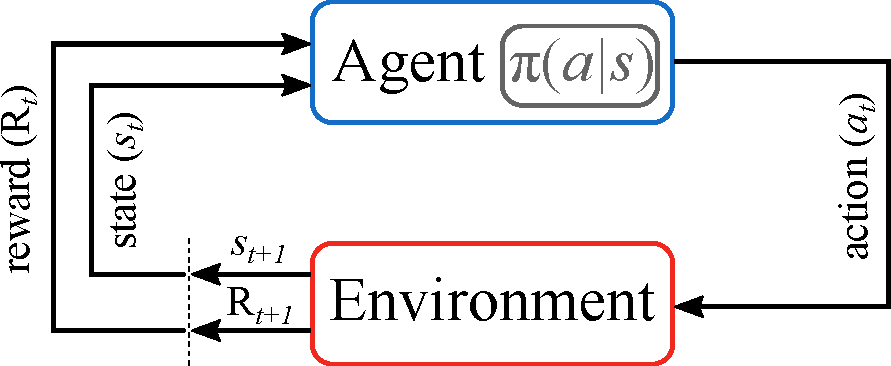
\includegraphics[width = 0.6\linewidth]{figures/RL_loop.pdf}
    \caption{Schematic of the typical learning loop for reinforcement learning agent. [Adapted from \citet{sutton2018reinforcement}]}
    \label{fig:RL_loop}
\end{figure}

In the previous description of the learning loop, $\mathcal{S}$, $\mathcal{A}$, and $\mathcal{R}$ correspond to the set of states, actions and rewards, respectively. These steps correspond to one cycle of the learning loop. The learning process extends for several cycles until a termination state is reached. The succession of cycles provides a repertory of actions and state observations ($s_t$ from now on for simplicity) that define a trajectory $\tau = (s_0,a_0,s_1,a_1,\dots)$. For each state, the agent looks for the optimal action to maximise its cumulative reward along the whole trajectory. In general, the targeted quantity is the discounted cumulative reward along a trajectory \citep{Viquerat2021RLrev}, defined as:
%
\begin{equation}
    R(\tau) = \sum_{t=0}^T \gamma^t r_t,
\end{equation}
%
where $T$ is the final time of the trajectory, and  $\gamma \in [0,1]$ is a discount factor to balance the relative importance of present and future rewards. The expected return is maximised through two possible approaches, namely value-based and policy-based methods. The former consist of determining the \textit{value function} \citep{sutton2018reinforcement} of a state-action pair, which is used to derive the following action to take at each state, while the latter directly aims at optimising a parameterised policy, which drives the agent performance.

A particularly successful application of RL is the resolution of games. The pioneering effort by \citet{Tesauro1992difflearn} describes a backgammon learner, in which the program started from no knowledge and trained by playing. After a million iterations, the program reached a performance similar to the best three human players in the world and won the computer backgammon olympiad \citep{BruntonNoackKoumoutsakos2020}. Recently, the development of neural networks allowed the application of RL to more complex games, such as Go \citep{mnih2015DRL} and the AI gym \citep{mnih2015DRL,Silver2016go}. RL is, however, a costly method due to the long learning process required to reach good performance. The acceleration of the learning process is a must for the application of RL to demanding scenarios, such as experiments and simulations of fluid flows \citep{Verma2018swimDRL}.

The agent does not only focus on revealing patterns in the environment dynamics or its actions but also aims at maximising the long-term rewards, which is the ultimate objective of RL methods. The long-term credit assignment (LTCA) implies assuming a certain relation between agent actions and environment rewards, which is derived from the trajectory of states and actions $\tau$. LTCA is still a major concern in RL. A common solution consists in modifying the original sparsely rewarded objective by adding highly rewarded sub-objectives \citep{schaul2015app}. Another challenge of RL is the correct use of information from experience by the agent when updated during the learning process \citep{Novati2019gliding}. In this regard, a proper tuning between \textit{exploration} and \textit{exploitation} is recommended. The agent must be able to find the optimal action by exploiting past experience while exploring alternative actions within the available solution space. Nonetheless, this is a common problem of several model-free algorithms.\\

Deep reinforcement learning (DRL) emerges from applying deep neural networks to model the agent. An artificial neural network (ANN), or simply neural network (NN), is a network of connected computational units, known as neurons, distributed in different layers that provides universal approximation capabilities \citep{Hornik1989MLP,Siegelmann1995NN}. For a fully connected network, each neuron receives input from all the neurons in the previous layer and feeds to all the neurons in the following layer. The neurons first compute the weighted sum of their inputs and, then, add a bias, which accounts for the output features that are independent of the input data. Eventually, the result from each neuron passes through a non-linear activation function that determines whether and to what extent the calculated value influences the final output. In DRL, NNs are trained to effectively map the relation between observations and actions \citep{rabault2019DRL}. This training process consists of the progressive adjustment of the biases and weights of the neural network towards the minimisation of a well-posed loss function that quantifies the network performance. The interested reader is referred to \citet{Goodfellow2016book} throughout the description of DRL.

In fluid mechanics, DRL has been recently applied to several problems to determine the parameters of control laws, such as swimming of fish schoolings \citep{gazzola2014RL}, control of unmanned aerial vehicles \citep{bohn2019DRL}, and optimization of glider trajectory taking ascendance \citep{reddy_learning_2016}. Most recently, DRL has been also applied to feedback-loop flow control like the wake control of a cylinder in simulations \citep{rabault2019DRL,rabault2019JFM} and in experiments \citep{Fan2020}, the tuning of the heat transport in a two-dimensional Rayleigh–Benard convection \citep{Beintema2020controlRBC}, and the wake stabilization past a cylinder by imposing a rotation on two control cylinders located at both sides \citep{Xu2020joh}.

\subsection{Policy-based methods} \label{ss:policymethods}
%
Policy methods rely on a \textit{policy} to drive the decision-making process of the agent. The final goal is to optimise the policy to maximise the expected discounted cumulative reward. The policy $\pi(a|s)$ is a mapping function based on a probability distribution over actions given a state rather than on a value function. Compared to value-based methods, policy-based methods ensure a better convergence, deal with high-dimensional action spaces, and exhibit great capabilities for learning stochastic policies \citep{Viquerat2021RLrev}. 

In fluid mechanics, most of the up-to-date applications of reinforcement learning prefer policy gradient methods, in which the parameterised policy $\pi_\theta(a|s)$ is optimised through a gradient ascent algorithm. The optimisation problem builds around the objective function, which is generally based on the expected discounted cumulative reward,
%
\begin{equation}
    J(\theta) = {\underset{\tau \sim \pi_\theta}{\mathbb{E}}}\left[ R(\tau) \right]
\end{equation}
%
to find the optimal set of parameters $\theta^*$ that maximises $J(\theta)$, namely
%
\begin{equation}
    \theta^* = {\underset{\theta}{\arg\max}}~{\underset{\tau \sim \pi_\theta}{\mathbb{E}}}\left[ R(\tau) \right]
\end{equation}

The optimisation problem could be directly solved by gradient ascent algorithm, considering an estimation of the policy gradient $\nabla_\theta J(\theta)$. The gradient with respect to the policy parameters $\theta$ is, however, a complex quantity to be determined. The common approach follows the log-probability trick \citep{Williams1992ML}, which derived $\nabla_\theta J(\theta)$ as an expected value that can be evaluated:
%
\begin{equation}
    \nabla_\theta J(\theta) = {\underset{\tau \sim \pi_\theta}{\mathbb{E}}}\left[ \sum_{t=0}^T \nabla_\theta \log(\pi_\theta(a_t|s_t)) R(\tau) \right],
\end{equation}

The evaluated gradient updates the policy parameters ($\theta \leftarrow \theta + \lambda  \nabla_\theta J(\theta)$, being $\lambda$ the learning rate) and the process repeats until convergence. The performance of policy gradient methods is jeopardised by the learning rate, which determines the step size in the gradient direction \citep{Viquerat2021RLrev}. Low learning rates translate into a long training process with no practical convergence whereas an excessive value of the learning rate could pass without heeding through the global optima, collapsing in a sub-optimal policy with poor performance. Proximal policy optimization \citep[PPO,][]{schulman_proximal_2017} relies on an effective heuristic to avoid destructive updates of the policy, i.e. it ensures restrained updates of the policy $\pi_\theta$, with respect to the previous $\pi_{\theta_{\text{old}}}$. The PPO method has drawn a lot of interest in the DRL community because of its increased learning stability and generally stable behaviour concerning hyperparameters. In fluid mechanics, early attempts to apply DRL for flow control focused on the simple problem of a shedding wake of a cylinder in simulations \citep{rabault2019JFM} and in experiments \citep{Fan2020}.

%------------------------------------------------------------------------------------------------
\section{Evolutionary Algorithms}

Optimization (and search) algorithms could be defined as learning algorithms featured by the determination of a probability distribution containing the relevant design aspects to optimise a given environment phenomenon \citep{BruntonNoackKoumoutsakos2020}. This conception was first envisioned by \citet{Schwefel1977}, introducing the concept of evolution strategies (ES) that later expanded to genetic algorithms \citep[GAs,][]{holland1992adaptation} and genetic programming \citep[GP,][]{Koza1994gp}, giving rise to the category of Evolutionary Algorithms (EA) in computational intelligence. Evolutionary algorithms or strategies build on the adaptation and progressive improvement of a set of candidate solutions inspired by biological evolution. Each potential solution is defined as an \textit{individual}, composing the \textit{population} that progressively evolves from one generation to the next. Darwin's ``evolution of species'' theory and its most recent updates and corrections describe the natural mechanisms governing the adaptation capability of individuals. The three main working principles of evolutionary algorithms derive from this knowledge \citep{duriez2017book,cornejomacedaPhD}, namely 
%
\begin{itemize}
    \item \textbf{survival of the best}: the most fitting or most performing individual, based on the environment requirements, prevails in the following generation. This mechanism guarantees the quality of incoming populations;
    \item \textbf{crossover}: mechanism to diversify the population by recombining individuals, which exploits the most performing features of the individuals;
    \item \textbf{mutation}: purely exploitative mechanism in which new individuals or features come up, ensuring uniqueness and freshness in following generations.
\end{itemize}
%
The recombination and mutation of individuals is a stochastic mechanism that guarantees the continuous exploitation and exploration of the most performing individuals within the solution space. Therefore, evolutionary algorithms may be thought of as crossbreeds between Monte Carlo sampling techniques, which explore the search space, and gradient search strategies, which exploit the best features toward a minimum.

Evolutionary algorithms can be used for flow control applications solving the optimisation problem in section~\ref{ss:optproblem}. The performance of each control law described by each individual is modelled by the cost function $J$ and the generation of individuals depends on the input data and the kind of algorithm. Under the umbrella of evolutionary algorithms, there is a wide variety of techniques to solve different types of problems. Some well-established examples are the genetic algorithms (GA) \citep{holland1992adaptation}, covariance matrix adaptation evolution strategy \citep{Hansen1996cmaes} or genetic programming (GP) \citep{Koza1994gp}. In this thesis, both GP and GA are considered in Papers 4 and 5, respectively. Both techniques stand on the same principle, mimicking natural processes; however, the definition of the individuals is different. GA identify the optimal individual as the best set of control parameters within the solution space, whereas GP derives a control law as a function of the input data, namely the sensor information. The control law provided by GP is commonly more complex and variable in time since it adjusts based on the state of the plant. GP represents a potent regression approach capable of re-discovering and combining flow control techniques without the need for physics knowledge in the circumstances of multi-frequency forcing and direct feedback control \citep{cornejomaceda2019pamm}.

GAs have been recently used to reduce the skin-friction drag in a TBL by optimising the phase delay among six streamwise-aligned slot jets \citep{Yu2021GA_drag_slot_jets},  to control the wake of a bluff body based on multi-frequency forcing \citep{minelli2020lgac}, and to optimise the performance of a spiral double-pipe heat exchanger \citep{Tian2020GAheatexchanger}, to name a few. In the field of heat transfer, the extensive review by \citet{Gosselin2009GareviewHT} describes many other successful applications of GA control. On the other hand, GP derives laws of low to medium complexity, such as the phasor control, threshold-level based control, periodic or multi-frequency forcing, including jet mixing optimization with pulsed jets at the nozzle exit \citep{zhou2020artificial}, drag reduction past bluff bodies \citep{li2019prf}, shear flow separation control \citep{gautier2015MLC}, reduction of vortex-induced vibrations of a cylinder \citep{Ren2019pof}, mixing layer control \citep{Parezanovic2016jfm}, and wake stabilization of complex shedding flows \citep{raibaudo2019pof}, among others.\\

The following section focuses on genetic programming, in particular in the Linear-based Genetic Programming (LGP) algorithm proposed by \citet{li2017GP} due to its greater degree of complexity compared to a classic GA. A brief description of the method and the learning process is provided. The interested reader on GAs is referred to \citet{holland1992adaptation} and \citet{Wahde2008book}.

\subsection{Genetic Programming}\label{ss:GP}
%
Genetic programming is an optimisation algorithm that proposes solution candidates as a computer program \citep{Koza1994gp}. These programs define the solutions in the form of a mathematical function of the input data, which could be used for several purposes such as fitting a surface, control laws or conditional decision making. In this section, this method is briefly introduced based on \citet{Wahde2008book}, \citet{duriez2017book} and \citet{cornejomacedaPhD}.

The internal representation of the mathematical function describing the control law is crucial to correctly applying the genetic operators. The classic classification distinguishes
%
\begin{itemize}
    \item \textbf{tree-based genetic programming}: the control law builds on a tree in which the nodes are the operators and the leaves are the operands \citep{duriez2017book}.
    \item \textbf{linear genetic programming (LGP)}: the control law is defined as a sequence of unitary or binary mathematical operations encoded in a matrix \citep{brameier2007linear}.
\end{itemize}
%
Despite sharing the same fundamental principle of operation, LGP is preferred in this thesis for its simplicity regarding multiple-input-multi-output (MIMO) control, since LGP deals with different input data and defines several control laws with only one matrix, and genetic operators, because mutation and crossover operations apply on the same matrix with simple combination or modification of individuals.

Linear genetic programming control (LGPC) is the application of LGP to solve control problems, deriving control laws as mathematical functions of the input data. The individuals, namely the control laws, are defined based on instructions, a register of variables and a set of constants \citep{duriez2014MLC}. The instructions combine input data through basic operations $(+,-,\times,\div,\sin,\text{exp},\text{\etc})$ to produce the control commands as outputs. Each individual, and its instructions, are represented by a 4-column matrix in which every row corresponds to an instruction. Columns 1 and 2 contain the register indices of the arguments, column 3 is the operator index, and column 4 is the output register. The registers are crucial in terms of memory management, distinguishing two types: \textit{variable registers} that can be overwritten during the execution of an instruction, commonly employed for intermediate calculations; and \textit{constant registers} that are preserved while the algorithms access the matrix data, which contain data of the problem or random constants. A potential problem of the matrix representation of the individual is the repetition of the same mathematical function after applying all the instructions, i.e. there is no unique matrix representation for a certain control law. A numerical test is performed before the evaluation of individuals in which repeated instances are discarded and replaced by a new one.

The combination of arguments and operators may yield instructions without any impact on the resultant control command, which is named \textit{introns}. These introns become crucial in the process of building relevant structures \citep{cornejomacedaPhD}. Nonetheless, the crossover and mutation operators may `activate' these instructions leading to an alteration of the resultant control law \citep{duriez2017book}. In principle, any mathematical function could be represented in matrix form if a sufficient number of instructions is considered together with a proper diversity in the operators' library. Not only that, but the library of input data plays a key role when building the proper control law. Eventually, the diversity of both libraries determines the complexity of the feasible solution space in the optimisation problem. \\

The LGPC process is described in the following as illustrated in figure~\ref{fig:GPC_algorithm}. The first step consists of a Monte Carlo optimisation through which a random sampling of individuals is used to generate the first population. Then, a tournament selection is carried out on the most performing individuals on which the genetic operations are performed to build the new generations. This process is repeated till convergence or when the stropping criterion is reached. Replication and elitism ensures the memory of the learning process while crossover and mutation exploit and explore over the solution space. The operator is chosen based on their respective probabilities ($P_c,P_m,P_r$), which are user-defined parameters that can be tuned to strengthen either the exploration or exploitation nature of the algorithm.

\begin{figure}
    \centering
    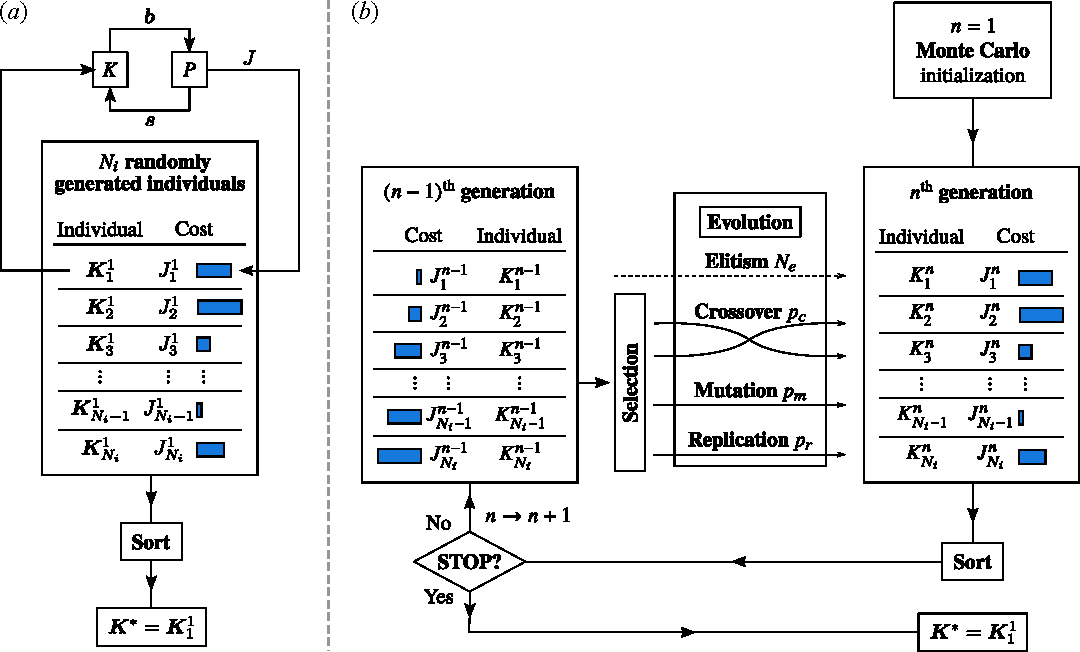
\includegraphics[width=0.99\linewidth]{figures/GPC_algorithm.pdf}
    \caption{(a) Monte Carlo sampling of the first generation. (b) Linear evolutionary algorithm. Each generation is built from the previous based on the genetic operators. \textit{Figures reproduced from \citet{cornejomacedaPhD} with permission of the author.}}
    \label{fig:GPC_algorithm}
\end{figure}

\subsubsection*{Monte Carlo optimisation}
Monte Carlo optimisation could, in principle, solve the flow control without the need for the evolutionary part; however, for a solution space with infinite dimensions, a multitude of individuals is required to ensure convergence toward the global optimum of the problem. LGPC considerably reduces the number of evaluations required for convergence, which becomes a limiting factor in real-life applications. The Monte Carlo optimization process provides the $N_i$ individuals of the first generation in the LGPC process by a random selection of operators and input data from the available libraries. Figure~\ref{fig:GPC_algorithm}(a) illustrate the Monte Carlo process for controlling a plant $P$ with the control law $K$ and control command $b$ (the reader is referred to section~\ref{ss:optproblem} for the definition of symbols). The maximum number of instructions and the number of variable and constant registers are user-defined parameters that the Monte Carlo sampling needs to comply with. The individuals are then evaluated and sorted based on their cost $J$. Eventually, the outcome of the algorithm is the most performing individual, i.e. the individual with the lowest cost.

\subsubsection*{Selection}
The genetic operations to build the incoming generations are performed on a certain set of individuals selected in a tournament selection process. The best $N_t$ individuals in the population are selected. The one that performs the best among them is picked with a probability of $P_t$. If not chosen, the same probability $P_t$ is used to select the second best and the process is repeated if needed for all the tournament individuals until the selection of the least performing. The user-defined parameters $N_t$ and $P_t$ influence the so-called \textit{selection pressure}, which is the degree to which high performers are chosen over low performers \citep{Wahde2008book}. Papers 4 and 5 in this thesis, for GP and GA respectively, follow the recommendations from \citet{duriez2017book}, setting $N_t = 7$ for a population of $N_i = 100$ individuals and $P_t = 1$.

\subsubsection*{Crossover for exploitation}
Crossover recombines individuals to extract the relevant features in the population. Thus, this is an exploitation operator through which two matrices split in two and swap, yielding two new individuals, namely the \textit{offsprings}.

\subsubsection*{Mutation for exploration}
The mutation is an exploitative operator to explore other features for a better control law. Each instruction has a certain probability to be randomly modified, which changes the matrix and, hence, leads to a new individual.

\subsubsection*{Replication and elitism for memory}
The most relevant features within a population are to be maintained for the incoming generation. Replication is the operator that copies individuals, ensuring the reminiscence of good individuals while enabling their future recombination. Similarly, the most performing individual during the process is always present in the latest generation due to elitism operator, preventing the loss of talent throughout the generations.
